    \documentclass[12pt, a4paper]{report}

\usepackage{elegant-cours}

\begin{document}

\MaPageDeGarde{Chapitre VII : Dérivation}{Rédigé par Samy Youssoufine}{./assets/logo.png}{Document WIP. Peut contenir des erreurs/sections incomplètes. Version ALPHA de la nouvelle mise en forme.}

\tableofcontents
\clearpage

\chapter{Généralités}

\begin{importantbox}
    Dans ce chapitre, $\mathbb{K}$ désigne soit $\R$ soit $\C$.
\end{importantbox}

\section{Dérivée en un point}

\begin{definition}[Dérivabilité en un point]
    Soient $I$ un intervalle de $\R$ tel que $\overset{\circ}{I}\neq\emptyset$ et $f\in\mathbb{K}^I$.

    On dit que $f$ est dérivable en $a \in I$ si et seulement si la fonction $\varphi$ définie par : $\begin{cases}I-\{a\}\to\mathbb{K}\\x\mapsto \frac{f(x)-f(a)}{x-a}\end{cases}$ admet une limite finie en $a$.

    Dans ce cas, la limite est appelée le nombre dérivé de $f$ en $a$ et est notée $f'(a)$.

    $$f'(a) = \lim_{x\to a} \frac{f(x)-f(a)}{x-a}$$
\end{definition}

\begin{remark}
    \begin{enumerate}
        \item $\lim_{x\to a} \frac{f(x)-f(a)}{x-a} = \lim_{h\to 0} \frac{f(a+h)-f(a)}{h}$
        \item Si $f \in \C^I$ tel que $f = f_1+if_2$ avec $f_1, f_2 \in \R^I$, alors $f$ est dérivable en $a$ si et seulement si $f_1$ et $f_2$ sont dérivables en $a$.\\Dans ce cas, $f'(a) = f_1'(a) + if_2'(a)$.\\On décompose la limite comme suit : $\lim_{x\to a} \frac{f(x)-f(a)}{x-a} = \lim_{x\to a} \frac{f_1(x)-f_1(a)}{x-a} + i\lim_{x\to a} \frac{f_2(x)-f_2(a)}{x-a}$
    \end{enumerate}
\end{remark}

\begin{definition}
    Soient $f \in \R^I$ et $a \in \overset{\circ}{I}$.
    
    On dit que $f$ est dérivable à gauche (resp. à droite) en $a$ ssi. la fonction $\varphi$ définie par : $\begin{cases}I\cap]-\infty,a[\to\R\\x\mapsto \frac{f(x)-f(a)}{x-a}\end{cases}$ (resp. $\begin{cases}I\cap]a,+\infty[\to\R\\x\mapsto \frac{f(x)-f(a)}{x-a}\end{cases}$) admet une limite finie en $a$.

    On peut aussi utiliser la notion de restriction pour définir la dérivabilité à gauche et à droite. Ainsi, $f$ est dérivable à gauche (resp. à droite) en $a$ si et seulement si la restriction de $f$ à $I\cap]-\infty,a[$ (resp. $I\cap]a,+\infty[$) est dérivable en $a$. 
    
    On peut donc écrire : $f$ dérivable à droite (resp. à gauche) en $a$ $\iff f_{|I\cap]a,+\infty[}$ (resp. $f_{|I\cap]-\infty,a[}$) dérivable en $a$.
\end{definition}

\begin{property}
    Soient $f \in \Kset^I$ et $a \in \overset{\circ}{I}$. On dit que $f$ est dérivable en $a$ si et seulement si $f$ est dérivable à gauche et à droite en $a$. De plus, dans ce cas, on a : $f'(a) = f'_{g}(a) = f'_{d}(a)$.
\end{property}

\begin{remark}
    \begin{enumerate}
        \item Si $f$ est une fonction à valeurs réelles telle que $f$ est dérivable à droite et à gauche en $a \in \overset{\circ}{I}$, avec $f'_{g}(a) \neq f'_{d}(a)$, alors $f$ n'est pas dérivable en $a$.\\Graphiquement, cela correspond à un angle (point anguleux) au point $a$. Voir la figure \ref{fig:point_anguleux}.
    \end{enumerate}
\end{remark}

\begin{figure}[H]
    \centering
    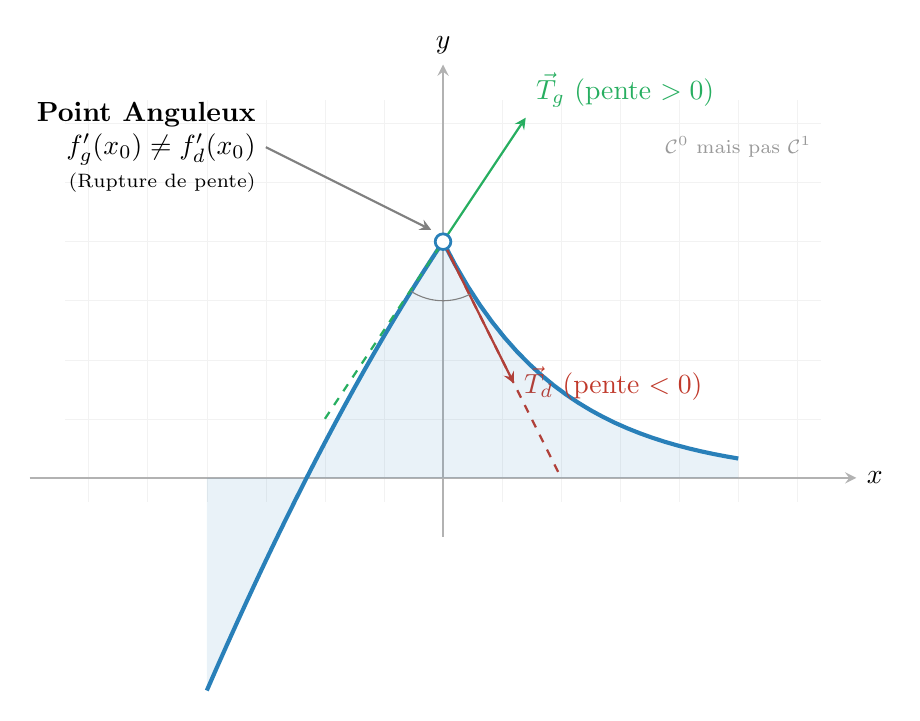
\begin{tikzpicture}[scale=1.5, >=stealth]
        % --- CONFIGURATION ---
        \definecolor{mainCurve}{RGB}{41, 128, 185}   % Bleu Nice
        \definecolor{tanLeft}{RGB}{39, 174, 96}      % Vert Émeraude
        \definecolor{tanRight}{RGB}{192, 57, 43}     % Rouge Foncé
        \definecolor{accent}{RGB}{241, 196, 15}      % Jaune

        % Grille d'arrière-plan discrète
        \draw[step=0.5, gray!10, very thin] (-3.2,-0.2) grid (3.2, 3.2);

        % Axes
        \draw[->, gray!60, thick] (-3.5,0) -- (3.5,0) node[right, black] {$x$};
        \draw[->, gray!60, thick] (0,-0.5) -- (0,3.5) node[above, black] {$y$};

        % --- FONCTIONS ---
        % But : Créer un "Pic" (Concave partout, mais cassure au sommet)
        % Partie Gauche (x < 0) : Parabole concave, pente à l'origine = +1.5
        % f(x) = 2 - (x - 1.5x) ... approximation quadratique
        % On utilise f(x) = 2.5 - 0.5(x-1)^2 -> Sommet en 1, donc montante en 0.
        % Simplifions : f(x) = 2 + 1.5x - 0.5x^2 pour x < 0. f(0)=2, f'(0)=1.5
        \draw[line width=1.5pt, mainCurve, domain=-2:0] plot (\x, {2 + 1.5*\x - 0.2*\x*\x});

        % Partie Droite (x > 0) : Exponentielle décroissante brutale, pente à l'origine = -2
        % f(x) = 2 * exp(-x). f(0)=2, f'(0)=-2.
        \draw[line width=1.5pt, mainCurve, domain=0:2.5] plot (\x, {2 * exp(-\x)});

        % --- DÉRIVÉES (DEMI-TANGENTES) ---
        % Tangente Gauche (Pente +1.5)
        \draw[tanLeft, dashed, thick] (-1, 0.5) -- (0, 2);
        \draw[->, tanLeft, thick] (0, 2) -- (0.7, 3.05) node[above right] {$\vec{T}_g$ (pente $>0$)};

        % Tangente Droite (Pente -2)
        \draw[tanRight, dashed, thick] (0, 2) -- (1, 0); 
        \draw[->, tanRight, thick] (0, 2) -- (0.6, 0.8) node[right] {$\vec{T}_d$ (pente $<0$)};

        % --- MISE EN FORME "CLASSE" ---
        % Remplissage sous courbe pour l'effet de volume
        \fill[mainCurve, opacity=0.1] 
            (-2,0) -- plot[domain=-2:0] (\x, {2 + 1.5*\x - 0.2*\x*\x}) 
            -- plot[domain=0:2.5] (\x, {2 * exp(-\x)}) 
            -- (2.5,0) -- cycle;

        % Le Point Anguleux
        \node[circle, fill=white, draw=mainCurve, line width=1pt, inner sep=2pt] (P) at (0,2) {};
        
        % Angle entre les tangentes (Visualisation de la non-dérivabilité)
        \draw[gray, thin] (0, 1.5) arc (270:297:0.5); % Juste décoratif
        \draw[gray, thin] (0, 1.5) arc (-270:-303:-0.5); % Juste décoratif
        
        % Annotation Latérale
        \draw[<-, thick, gray] (-0.1, 2.1) -- (-1.5, 2.8) node[left, align=right, text=black] {
            \textbf{Point Anguleux}\\
            $f'_g(x_0) \neq f'_d(x_0)$\\
            \scriptsize{(Rupture de pente)}
        };

        % Formule indicative (optionnel, pour faire "pro")
        \node[text=gray!80, font=\scriptsize] at (2.5, 2.8) {$\mathcal{C}^0$ mais pas $\mathcal{C}^1$};

    \end{tikzpicture}
    \caption{Représentation graphique d'une fonction continue non dérivable en $x=0$. Le changement brusque de la pente (de positive à gauche à négative à droite) crée un point anguleux caractéristique.}
    \label{fig:point_anguleux}
\end{figure}

\section{Fonctions dérivées}

\begin{definition}
    Soit $f\in \Kset^I$. On dit que $f$ est dérivable sur $I$ lorsque $f$ est dérivable en $a$ pour tout $a \in I$.

    Dans ce cas, on définit la fonction dérivée de $f$ sur $I$ comme la fonction :

    $$f' : \begin{cases}I\to\Kset\\x\mapsto f'(x)\end{cases}$$

    On note l'ensemble des fonctions dérivables sur $I$ par $\mathcal{D}(I,\Kset)$, ou encore $\mathcal{D}^1(I,\Kset)$
\end{definition}

\begin{property}
    Soit $f \in \Kset^I$.
    \begin{enumerate}
        \item Si $f$ est dérivable en $a$, alors $f$ est continue en $a$ (La réciproque est fausse !).
        \item Si $f$ est dérivable sur $I$, alors $f$ est continue sur $I$.\\On peut donc écrire : $f \in \mathcal{D}(I,\Kset) \implies f \in \mathcal{C}(I,\Kset)$, et encore $\mathcal{D}^1(I,\Kset) \subset \mathcal{C}^0(I,\Kset)$.
    \end{enumerate}
\end{property}

\begin{proof}
    Soit $f \in \Kset^I$ dérivable en $a \in I$. 

    On pose $\varphi : \begin{cases}I-\{a\}\to\Kset\\x\mapsto \begin{cases}
\frac{f(x)-f(a)}{x-a} & \text{si } x \neq a\\
f'(a) & \text{si } x = a
    \end{cases}\end{cases}$.

    Comme f est dérivable en $a$, $\varphi$ est continue en $a$.

    On a donc $\forall x\in I, f(x)=\varphi(x)(x-a)+f(a)$.

    Donc $\lim_{x\to a} f(x) = \lim_{x\to a} \varphi(x)(x-a)+f(a) = f(a)$.

    Ainsi, $f$ est continue en $a$.
\end{proof}

\begin{remark}
    \begin{outline}
        \1 La réciproque de la propriété précédente est fausse.

        \2 Par exemple, la fonction $x\mapsto |x|$ est continue mais non-dérivable en $0$.
        
        \2 On peut aussi voir que la fonction illustrée dans la figure \ref{fig:point_anguleux} est continue mais non-dérivable en $0$.

        \1 Certaines fonctions sont continues partout mais non dérivables partout, comme la fonction de Weierstrass, ou celle du mouvement brownien en probabilité. Voir la figure \ref{fig:weierstrass_function} pour une illustration de la fonction de Weierstrass.
    \end{outline}
\end{remark}

% figure de la fonction de Weierstrass
\begin{figure}[H]
    \centering
    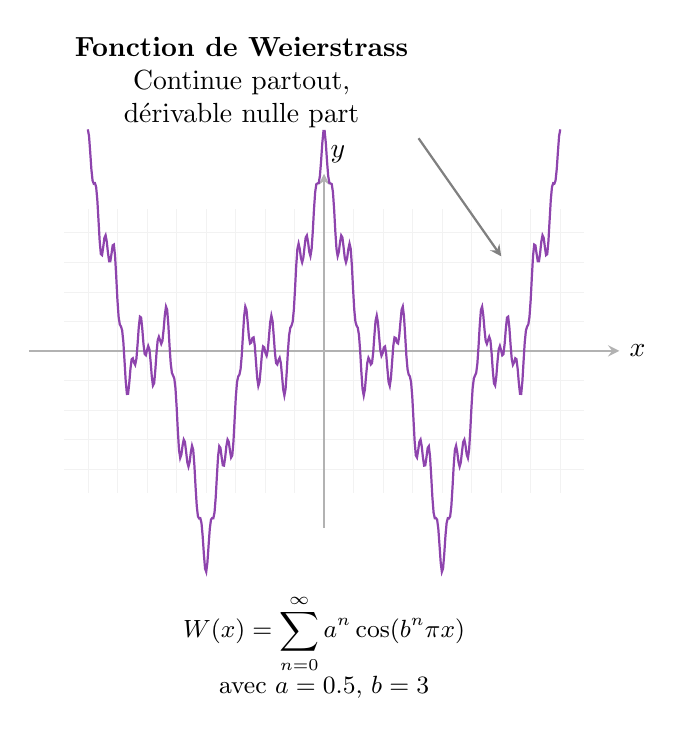
\begin{tikzpicture}[scale=1.5, >=stealth]
        % --- CONFIGURATION ---
        \definecolor{weierstrassCurve}{RGB}{142, 68, 173}   % Violet Nice
        \definecolor{accent}{RGB}{241, 196, 15}      % Jaune

        % Grille d'arrière-plan discrète
        \draw[step=0.25, gray!10, very thin] (-2.2,-1.2) grid (2.2, 1.2);

        % Axes
        \draw[->, gray!60, thick] (-2.5,0) -- (2.5,0) node[right, black] {$x$};
        \draw[->, gray!60, thick] (0,-1.5) -- (0,1.5) node[above, black] {$~~~y$};

        % --- FONCTION DE WEIERSTRASS (APPROXIMATION SIMPLIFIÉE) ---
        % W(x) = sum_{n=0}^{infty} a^n * cos(b^n * pi * x)
        % Avec a = 0.5, b = 3 (approximation avec moins de termes pour éviter l'overflow)
        \draw[weierstrassCurve, thick, domain=-2:2, samples=400] plot (\x, {
            cos(deg(pi * \x)) + 
            0.5 * cos(deg(3 * pi * \x)) + 
            0.25 * cos(deg(9 * pi * \x)) + 
            0.125 * cos(deg(27 * pi * \x))
        });

        % Formule de la fonction
        \node[align=center, font=\small] at (0, -2.5) {
            $W(x) = \displaystyle\sum_{n=0}^{\infty} a^n \cos(b^n \pi x)$\\
            avec $a = 0.5$, $b = 3$
        };

        % Annotation Latérale
        \draw[<-, thick, gray] (1.5, 0.8) -- (0.8, 1.8) node[above left, align=center, text=black] {
            \textbf{Fonction de Weierstrass}\\
            Continue partout,\\
            dérivable nulle part
        };
    \end{tikzpicture}
    \caption{Représentation graphique de la fonction de Weierstrass $W(x) = \sum_{n=0}^{\infty} a^n \cos(b^n \pi x)$ avec $a = 0{,}5$ et $b = 3$. Cette fonction est continue partout mais n'est dérivable en aucun point.}
    \label{fig:weierstrass_function}
\end{figure}

\section{Opérations sur les fonctions dérivables}

\begin{property}
    \label{prop:operations_derivables}
    Soient $f,g \in \mathcal{D}(I,\Kset)$.

    \begin{enumerate}
        \item $\forall \lambda \in \Kset, \lambda f + g \in \mathcal{D}(I,\Kset)$ et $(\lambda f + g)' = \lambda f' + g'$
        \item $fg \in \mathcal{D}(I,\Kset)$ et $(fg)' = f'g + fg'$
        \item Si $g$ ne s'annule pas sur $I$, alors $\frac{f}{g} \in \mathcal{D}(I,\Kset)$ et $\left(\frac{f}{g}\right)' = \frac{f'g - fg'}{g^2}$ et $\left(\frac{1}{g}\right)' = -\frac{g'}{g^2}$
    \end{enumerate}
\end{property}

\begin{proof}[Preuve de la propriété \ref{prop:operations_derivables} - 1.]
    Soit $a \in I$.
    \begin{align*}
        (\lambda f + g)'(a) &= \lim_{x\to a} \frac{(\lambda f + g)(x) - (\lambda f + g)(a)}{x-a} \\
        &= \lim_{x\to a} \frac{\lambda (f(x) - f(a)) + (g(x) - g(a))}{x-a} \\
        &= \lambda \lim_{x\to a} \frac{f(x) - f(a)}{x-a} + \lim_{x\to a} \frac{g(x) - g(a)}{x-a} \\
        &= \lambda f'(a) + g'(a)
    \end{align*}
\end{proof}

\begin{proof}[Preuve de la propriété \ref{prop:operations_derivables} - 2.]
    Soit $a \in I$.
    \begin{align*}
        (fg)'(a) &= \lim_{x\to a} \frac{f(x)g(x) - f(a)g(a)}{x-a} \\
        &= \lim_{x\to a} \frac{f(x)g(x) - f(a)g(x) + f(a)g(x) - f(a)g(a)}{x-a} \\
            &= \lim_{x\to a} g(x)\frac{f(x) - f(a)}{x-a} + f(a)\lim_{x\to a} \frac{g(x) - g(a)}{x-a} \\
            &= g(a)f'(a) + f(a)g'(a)
    \end{align*}
\end{proof}
    
\begin{proof}[Preuve de la propriété \ref{prop:operations_derivables} - 3.]
    Soit $a \in I$.
    \begin{align*}
        \left(\frac{f}{g}\right)'(a) &= \lim_{x\to a} \frac{\frac{f(x)}{g(x)} - \frac{f(a)}{g(a)}}{x-a} \\
            &= \lim_{x\to a} \frac{f(x)g(a) - f(a)g(x)}{(x-a)g(x)g(a)} \\
            &= \lim_{x\to a} \frac{g(a)(f(x)-f(a)) - f(a)(g(x)-g(a))}{(x-a)g(x)g(a)} \\
            &= \frac{g(a)f'(a) - f(a)g'(a)}{g(a)^2} \\
            &= \frac{f'(a)g(a) - f(a)g'(a)}{g(a)^2}
    \end{align*}
\end{proof}

\begin{proof}[Preuve de la propriété \ref{prop:operations_derivables} - 4.]
    Soit $a \in I$.
    \begin{align*}
        \left(\frac{1}{g}\right)'(a) &= \lim_{x\to a} \frac{\frac{1}{g(x)} - \frac{1}{g(a)}}{x-a} \\
            &= \lim_{x\to a} \frac{g(a) - g(x)}{(x-a)g(x)g(a)} \\
            &= \lim_{x\to a} \frac{-(g(x)-g(a))}{(x-a)g(x)g(a)} \\
            &= -\frac{g'(a)}{g(a)^2} ~~ \text{car } \frac1g \text{ est continue en } a
    \end{align*}
\end{proof}

\begin{example}
    \begin{enumerate}
        \item Soit $f \in \mathcal{D}(I,\Kset)$. On pose $g:x\mapsto f(x)e^x$.\\On a $g$ est dérivable sur $I$ avec $\forall x \in I, g'(x) = f'(x)e^x + f(x)e^x = (f'(x) + f(x))e^x$.
        \item Soit $P:x\mapsto \sum_{k=0}^{n}a_kx^k$ où $a_k \in \Kset$.\\On a $P \in \mathcal{D}(\R,\Kset)$ avec $\forall x \in \R, P'(x) = \sum_{k=1}^{n}ka_kx^{k-1}$.
    \end{enumerate}
\end{example}

\begin{property}
    Soit $f$ une fonction de $I$ vers $\C$.

    Alors $f$ est dérivable sur $I$ si et seulement si les fonctions parties réelles et imaginaires de $f$ sont dérivables sur $I$.

    Cela équivaut aussi à dire que $\overline{f}$ est dérivable sur $I$, et on a $\parens{\overline{f}}' = \overline{f'}$.
\end{property}

\begin{proof}
    On pose $f=f_1 + if_2$ avec $f_1, f_2 : I \to \R$.

    Si $f$ est dérivable sur $I$, alors $f_1$ et $f_2$ sont dérivables sur $I$ avec $\forall x \in I, f'(x) = f_1'(x) + if_2'(x)$.

    Ce qui implique que $\overline{f}(x) = f_1(x) - if_2(x)$ est dérivable sur $I$ avec $\forall x \in I, \parens{\overline{f}}'(x) = f_1'(x) - if_2'(x) = \overline{f'(x)}$.

    Réciproquement, si $f_1$ et $f_2$ sont dérivables sur $I$, alors $f$ est dérivable sur $I$ avec $\forall x \in I, f'(x) = f_1'(x) + if_2'(x)$.

    De plus, si $\overline{f}$ est dérivable sur $I$, alors $f_1$ et $f_2$ sont dérivables sur $I$ avec $\forall x \in I, \parens{\overline{f}}'(x) = f_1'(x) - if_2'(x)$.

    Ainsi, $f$ est dérivable sur $I$ avec $\forall x \in I, f'(x) = f_1'(x) + if_2'(x) = \overline{\parens{\overline{f}}'(x)}$.
\end{proof}

\begin{property}
    Soient $f \in \mathcal{D}(I,\R)$ et $g \in \mathcal{D}(J,\Kset)$ avec $f(I) \subset J$.

    Alors la composée $g\circ f$ est dérivable sur $I$ avec $\forall x \in I, (g\circ f)'(x) = g'(f(x)) \cdot f'(x)$.

    \begin{attention}
        Il est important de noter que cette propriété nécessite que $f$ soit dans $\mathcal{D}(I,\R)$ et non dans $\mathcal{D}(I,\Kset)$. En effet, la dérivabilité de $g\circ f$ n'est pas garantie si $f$ prend des valeurs complexes.
    \end{attention}
\end{property}

\begin{proof}
    Soit $a \in I$.
    \begin{align*}
        (g\circ f)'(a) &= \lim_{x\to a} \frac{g(f(x)) - g(f(a))}{x-a} \\
            &= \lim_{x\to a} \frac{g(f(x)) - g(f(a))}{f(x) - f(a)} \cdot \frac{f(x) - f(a)}{x-a} \\
            &= g'(f(a)) \cdot f'(a)
    \end{align*}
\end{proof}

\begin{exercise}
    Soit $f : I\to \C$ une fonction dérivable sur $I$, telle que $\forall x \in I, f(x)\not=0$.

    \begin{enumerate}
        \item Montrer que $\abs{f}$ est dérivable sur $I$.
        \item Calculer $(\abs{f})'(x)$ pour tout $x \in I$ en fonction de $\abs{f}$ et $f$.
    \end{enumerate}

    \textbf{Solution :}

    \begin{outline}[enumerate]
        \1 On veut montrer que la fonction $\abs{f} : \begin{cases} I \to \R \\ x \mapsto \abs{f(x)} \end{cases}$ est dérivable sur $I$.
        \2 Méthode 1 (Décomposer la fonction $f$ en $f_1 + if_2$) ;
        \3 On pose $f_1, f_2 : I \to \R$ telles que $\forall x \in I, f(x) = f_1(x) + if_2(x)$.
        \3 Comme $f$ est dérivable sur $I$, alors $f_1$ et $f_2$ sont dérivables sur $I$.
        \3 On a $\forall x \in I, \abs{f(x)} = \sqrt{f_1(x)^2 + f_2(x)^2}$.
        \3 On a $f_1(x)^2 + f_2(x)^2 > 0$ car $f(x) \neq 0$ (démonstration par absurde triviale).
        \3 On pose $g : \begin{cases} (0,+\infty) \to \R \\ t \mapsto \sqrt{t} \end{cases}$.
        \3 La fonction $g$ est dérivable sur $]0,+\infty[$.
        \3 Par composition, $\abs{f} = g \circ h$ avec $h : \begin{cases} I \to ]0,+\infty[ \\ x \mapsto f_1(x)^2 + f_2(x)^2 \end{cases}$ est dérivable sur $I$.
        \2 Méthode 2 (Utiliser la fonction conjugée) ;
        \3 On a $\forall x \in I, \abs{f(x)} = \sqrt{f(x)\overline{f(x)}}$.
        \3 On pose $g : \begin{cases} ]0,+\infty[ \to \R \\ t \mapsto \sqrt{t} \end{cases}$
        \3 Reste de la résolution quasi identique...
        \1 Calcul de la dérivée de $\abs{f}$.
        \2 On a $\forall x \in I, \abs{f(x)} = \sqrt{f(x)\overline{f(x)}}$.
        \2 On a alors $|f|'= \frac{f'\cdot\overline{f} + f\cdot(\overline{f})'}{2\sqrt{f\overline{f}}}$.
        \2 Or, $(\overline{f})' = \overline{f'}$.
        \2 Donc, $\forall x \in I, (\abs{f})'(x) = \frac{f'(x)\overline{f(x)} + f(x)\overline{f'(x)}}{2\abs{f(x)}}$.
        \2 On peut aussi écrire $(\abs{f})'(x) = \frac{\Re\parens{f'(x)\overline{f(x)}}}{\abs{f(x)}}$.
    \end{outline}

\end{exercise}

\begin{property}
    Soit $f:I\to J$ une bijection (donc $f(I)=J$).

    Si $f$ est dérivable en $a \in I$ avec $f'(a) \neq 0$, alors $f^{-1}$ est dérivable en $f(a)$ avec $\parens{f^{-1}}'(f(a)) = \frac{1}{f'(a)}$.
\end{property}

\begin{proof}
    \begin{align*}
        \lim_{y\to f(a)} \frac{f^{-1}(y) - f^{-1}(f(a))}{y - f(a)} &= \lim_{x\to a} \frac{f^{-1}(f(x)) - f^{-1}(f(a))}{f(x) - f(a)} \\
            &= \lim_{x\to a} \frac{x - a}{f(x) - f(a)} \\
            &= \frac{1}{\lim_{x\to a} \frac{f(x) - f(a)}{x - a}} \\
            &= \frac{1}{f'(a)}
    \end{align*}

    Sans oublier que $y \in J \implies y = f(x)$ avec $x \in I$ car $f$ est une bijection.
\end{proof}

\begin{remark}
    Si $f:I\to J$ dérivable sur $I$ telle que $\forall x \in I, f'(x) \neq 0$, alors $f^{-1}$ est dérivable sur $J$ avec $\forall y \in J, \parens{f^{-1}}'(y) = \frac{1}{f'(f^{-1}(y))}$.
\end{remark}

\begin{property}
    \begin{enumerate}
        \item Les fonctions $\arcsin$ et $\arccos$ sont dérivables sur $]-1,1[$.\\Et on a $\forall x \in ]-1,1[, \parens{\arcsin}'(x) = \frac{1}{\sqrt{1-x^2}}$ et $\parens{\arccos}'(x) = -\frac{1}{\sqrt{1-x^2}}$.
        \item La fonction $\arctan$ est dérivable sur $\R$ avec $\forall x \in \R, \parens{\arctan}'(x) = \frac{1}{1+x^2}$.
        \item $\argch$ est dérivable sur $]1,+\infty[$ avec $\forall x \in ]1,+\infty[, \parens{\argch}'(x) = \frac{1}{\sqrt{x^2-1}}$.
        \item $\argsh$ est dérivable sur $\R$ avec $\forall x \in \R, \parens{\argsh}'(x) = \frac{1}{\sqrt{1+x^2}}$.
        \item $\argth$ est dérivable sur $]-1,1[$ avec $\forall x \in ]-1,1[, \parens{\argth}'(x) = \frac{1}{1-x^2}$.
    \end{enumerate}
\end{property}

\begin{remark}
  On a $\forall x \in ]-1,1[, \arccos'(x) + \arcsin'(x)=0$.

  Donc $\arccos(x) + \arcsin(x) = C$ pour une certaine constante $C$.

  En évaluant en $x=0$, on trouve $C = \frac{\pi}{2}$.
  
  Cette égalité est conservée pour $x\in\{-1,1\}$.
\end{remark}

\begin{definition}[Dérivée $n$-ième]
	Soient $n\in\N*$ et $f\in\Kset^I$.
	
	$f$ est dite $\mathcal{D}^n$ sur $I$ lorsque $f$ est $n$-fois dérivable sur $I$, et on note la dérivée $n$-ième de $f$ par $f^{(n)}$

  On note $\mathcal{D}^n(I,\Kset)$ l'ensemble des fonctions $f\in\Kset^I$ $n$-fois dérivables sur $I$.
\end{definition}

\begin{remark}
	Il est important de noter que la notation de la composée $n$-ième ($f\circ f\circ \dots \circ f)$ a la même notation que la dérivée $n$-ième. Il faut donc faire attention au contexte !
\end{remark}

\begin{property}[Formule de Leibniz]
    Soient $f,g \in \mathcal{D}^n(I,\Kset)$.

    \begin{keyformula}
    $f\cdot g \in \mathcal{D}^n(I,\Kset)$ avec $\forall x \in I, (fg)^{(n)}(x) = \sum_{k=0}^{n} \legbinom{n}{k} f^{(k)}(x) g^{(n-k)}(x)$.
    \end{keyformula}
\end{property}

\begin{proof}
  Nous allons procéder à la démonstration par récurrence sur $n\in\N^*$.

  \textbf{Initialisation :} Pour $n=1$, la formule de Leibniz est donnée par la propriété des opérations sur les fonctions dérivables, qui stipule que $(fg)' = f'g + fg'$. La formule est donc vérifiée pour $n=1$.

  \textbf{Hérédité :} Soit $n \in \N^*$. Nous allons supposer que la propriété est vraie pour ce rang $n$.

  Soient $f,g \in \mathcal{D}^{n+1}(I,\Kset)$. Par hypothèse de récurrence, nous avons :
  \[(fg)^{(n)}(x) = \sum_{k=0}^{n} \legbinom{n}{k} f^{(k)}(x) g^{(n-k)}(x).\]

  On sait donc que $f,g\in\mathcal{D}^1(I,\Kset)$ et que $(fg)^{(n)} \in \mathcal{D}^1(I,\Kset)$, et $(f,g)'=fg'+f'g$.

  On sait que $f \in \mathcal{D}^{n+1}(I,\Kset)$ et $g \in \mathcal{D}^{n+1}(I,\Kset)$, donc $f \in \mathcal{D}^n(I,\Kset)$ et $g' \in \mathcal{D}^n(I,\Kset)$, donc $f'\cdot g\in \mathcal{D}^{n}(I,\Kset)$.

  On sait aussi que $f' \in \mathcal{D}^n(I,\Kset)$ et $g \in \mathcal{D}^n(I,\Kset)$, donc $f'\cdot g\in \mathcal{D}^{n}(I,\Kset)$.

  Donc $fg' + f'g \in \mathcal{D}^n(I,\Kset)$.

  D'après l'hypothèse de récurrence, on a :
  \begin{align*}
    (fg)^{(n+1)} &= ((fg)^{(n)})' \\
    &= \left(\sum_{k=0}^{n}\legbinom{n}{k} f^{(k)}\cdot g^{(n-k)}\right)' \\
    &= \sum_{k=0}^{n}\legbinom{n}{k} \left(f^{(k)}\cdot g^{(n-k)}\right)' \\
    &= \sum_{k=0}^{n}\legbinom{n}{k} \left(f^{(k+1)}\cdot g^{(n-k)} + f^{(k)}\cdot g^{(n-k+1)}\right) \\
    &= \sum_{k=0}^{n}\legbinom{n}{k} f^{(k+1)}\cdot g^{(n-k)} + \sum_{k=0}^{n}\legbinom{n}{k} f^{(k)}\cdot g^{(n-k+1)} \\
    &= \sum_{k=1}^{n+1}\legbinom{n}{k-1} f^{(k)}\cdot g^{(n+1-k)} + \sum_{k=0}^{n}\legbinom{n}{k} f^{(k)}\cdot g^{(n+1-k)} \\
    &= \legbinom{n+1}{0} f^{(0)}\cdot g^{(n+1)} + \sum_{k=1}^{n} \left(\legbinom{n}{k-1} + \legbinom{n}{k}\right) f^{(k)}\cdot g^{(n+1-k)} + \legbinom{n+1}{n+1} f^{(n+1)}\cdot g^{(0)} \\
    &= \sum_{k=0}^{n+1} \legbinom{n+1}{k} f^{(k)}\cdot g^{(n+1-k)}
  \end{align*}

  Ainsi, la formule de Leibniz est vérifiée pour $n+1$.

  Par le principe de récurrence, la formule de Leibniz est donc vérifiée pour tout $n \in \N^*$.
\end{proof}

\begin{remark}
    $f^{(0)} = f$ par convention.

    On ne peut pas parler d'une fonction "zéro-fois dérivable", mais la notation $f^{(0)}$ est utile pour exprimer des formules générales, comme la formule de Leibniz.
\end{remark}

\begin{example}
  \begin{enumerate}
    \item $\forall x \in \R, \sin^{(n)}(x) = \sin\parens{x + \frac{n\pi}{2}}$.
    \item $\forall x \in \R, \cos^{(n)}(x) = \cos\parens{x + \frac{n\pi}{2}}$.
    \item Soient $a\in\C$, $n\in\N$. On a $\forall x \in \R-\set{a}, (x\mapsto \frac1{x-a})^{(n)}(x)=\frac{(-1)^n n!}{(x-a)^{n+1}}$.
    \item Soient $k,n\in\N, a\in\C$.\\On a $\forall x \in \R, (x\mapsto (x-a)^k)^{(n)}(x) = \begin{cases}
        \frac{k!}{(k-n)!}(x-a)^{k-n} & \text{si } n \leq k\\
        0 & \text{si } n > k\end{cases}$
    \item $P:x\mapsto \sum_{k=0}^s a_kx^k$ avec $s\in\N$.\\On a $\forall j \in \set{0,\dots,s}, P^{(j)}(x) = \parens{\sum_{k=0}^s a_k x^k}^{(j)} \\= \sum_{k=0}^{j-1} a_k \underbrace{(x^k)^{(j)}}_{=0} + \sum_{k=j}^s a_k\underbrace{\parens{x^{k}}^{(j)}}_{=\frac{k!}{(k-j)!} x^{k-j}}$.\\Donc, $\forall j \in \set{0,\dots,s}, P^{(j)}(x) = \sum_{k=j}^s a_k \frac{k!}{(k-j)!} x^{k-j}$.\\Donc, pour tout $j\in\set{0,\dots,s}$, $P^{(j)}(0)=a_j\cdot \frac{j!}{1}\\ \implies a_j=\frac{P^{(j)}(0)}{j!}$
    \item On en déduit que $\forall x \in \R, P(x) = \sum_{k=0}^n \frac{P^{(k)}(0)}{k!} x^k$.\\Ou encore, $\forall a \in \R, \forall x \in \R, P(x) = \sum_{k=0}^n \frac{P^{(k)}(a)}{k!} (x-a)^k$.
  \end{enumerate}
\end{example}

\begin{remark}[Développement limité]
  Les deux derniers exemples forment la base du développement limité des fonctions en un point, qui sera vu plus en détail dans un prochain chapitre. Le développement limité consiste, en principe, à approcher une fonction par un polynôme de degré $n$ en un point donné, en utilisant les dérivées successives de la fonction à ce point. Il reste donc toujours une erreur pour des fonctions quelconques, mais les fonctions polynomiales sont parfaitement représentées par leur développement limité.
\end{remark}

\begin{definition}
  Soient $f \in \Kset^I$ et $a\in\N$.
  \begin{itemize}
    \item $f$ est dite de classe $\mathcal{C}^n$ sur $I$ lorsque $f^{(n)}$ existe et est continue sur $I$.
    \item On note l'ensemble des fonctions de classe $\mathcal{C}^n$ sur $I$ par $\mathcal{C}^n(I,\Kset)$.
    \item On dit que $f$ est de classe $\mathcal{C}^{\infty}$ sur $I$ lorsque $f$ est de classe $\mathcal{C}^n$ pour tout $n \in \N$.
    \item On note l'ensemble des fonctions de classe $\mathcal{C}^{\infty}$ sur $I$ par $\mathcal{C}^{\infty}(I,\Kset)$.
  \end{itemize}
\end{definition}

\begin{remark}
  \begin{enumerate}
    \item On a $\forall n \in \N^*, \mathcal{C}^n(I,\Kset) \subsetneq \mathcal{D}^n(I,\Kset) \subsetneq \mathcal{C}^{n-1}(I,\Kset)$ pour tout $n \in \N$.\\\textbf{Attention : il s'agit d'une inclusion stricte $\subsetneq \equiv \subset$ ! On note normalement les inclusions par $\subseteq$, mais dans ce cours, les inclusions non-strictes seront tout de même notées $\subset$}.
    \item $\mathcal{C}^0(I,\Kset) = \mathcal{C}(I,\Kset)$.
  \end{enumerate}
\end{remark}

\begin{example}
  $$f:x\mapsto \begin{cases}
  x^3\sin\parens{\frac1x} & \text{si } x \neq 0\\
  0 & \text{si } x = 0
  \end{cases}$$

  On a $\lim_{x \to 0} f(x) = 0 = f(0)$, donc $f$ est continue en $0$.

  On a $\lim_{x \to 0} \frac{f(x) - f(0)}{x - 0} = \lim_{x \to 0} x^2 \sin\parens{\frac1x} = 0$, donc $f$ est dérivable en $0$ avec $f'(0) = 0$.

  Donc $f$ est dérivable sur $\R$ avec $f'(x) = \begin{cases}
  3x^2\sin\parens{\frac1x} - x\cos\parens{\frac1x} & \text{si } x \neq 0\\0 & \text{si } x = 0\end{cases}$

  Donc $f$ est de classe $\mathcal{D}^1$ sur $\R$.

  On a $\lim_{x \to 0} f'(x) = \lim_{x \to 0} 3x^2\sin\parens{\frac1x} - x\cos\parens{\frac1x} = 0 = f'(0)$, donc $f'$ est continue en $0$.

  Donc $f$ est de classe $\mathcal{C}^1$ sur $\R$.

  En revanche, on peut démontrer que $f \notin \mathcal{D}^2(\R,\R)$ car $f'$ n'est pas dérivable en $0$.
\end{example}

\begin{property}
    Soient $f,g \in \mathcal{C}^n(I,\Kset)$.
    \begin{enumerate}
        \item $\forall \lambda \in \Kset, \lambda f + g \in \mathcal{C}^n(I,\Kset)$
        \item $f\cdot g \in \mathcal{C}^n(I,\Kset)$
    \end{enumerate}
\end{property}

\begin{proof}
  Preuves à refaire en tant qu'exercices.
\end{proof}

\begin{property}
  Soient $f\in\mathcal{C}^n(I,\R)$ et $g\in\mathcal{C}^n(J,\Kset)$ avec $f(I)\subset J$.

  \begin{importantbox}
    Alors $g\circ f \in \mathcal{C}^n(I,\Kset)$.
  \end{importantbox}
\end{property}

\begin{proof}
  Nous allons procéder par récurrence sur $n\in\N$.

  \textbf{Initialisation :} Pour $n=0$, la propriété est vraie car la composition de fonctions continues est continue (voir chapitre sur la continuité).

  \textbf{Hérédité :} Soit $n\in\N$. Nous allons supposer que la propriété est vraie pour ce rang $n$.

  Soit $f\in\mathcal{C}^{n+1}(I,\R)$ et $g\in\mathcal{C}^{n+1}(J,\Kset)$ avec $f(I)\subset J$.

  Donc, on a $f$ est $\mathcal{C}^1$ et $g$ est $\mathcal{C}^1$.

  Donc $g\circ f$ est dérivable sur $I$ avec $(g\circ f)' = f' (g'\circ f)$.

  Donc $f$ est $\cclas{n+1}$, ce qui implique que $f' \in \cclas{n}$.

  Donc, sachant que $g$ est $\cclas{n+1}$, donc $g' \in \cclas{n}$, et $f$ est $\cclas{n+1}$, donc $f'$ est $\cclas{n}$, par hypothèse de récurrence, on a $g'\circ f$ est $\cclas{n}$.

  Donc, $f'\cdot(g'\circ f)$ est $\cclas{n}$.

  Donc $g\circ f$ est $\cclas{n+1}$.
\end{proof}

\begin{property}
  Soit $f \in \cclas{n}(I,\Kset)$ telle que $f$ ne s'annule pas sur $I$. Alors $\frac1f \in \cclas{n}(I,\Kset)$.
\end{property}

\chapter{Étude globale}

\section{Extrémums locaux et globaux}

\begin{definition}
  Soient $f \in \R^I$ et $x_0 \in I$.

  Un extrémum de $f$ en $x_0$ est une valeur $f(x_0)$ telle que $f$ ne prend pas de valeur plus grande (respectivement, plus petite) que $f(x_0)$ à proximité de $x_0$. Plus simplement, un extremum est un point où la fonction atteint un "pic" (maximum) ou un "creux" (minimum).

  On dit que $x_0$ est un minimum (respectivement, un maximum) local de $f$ lorsque :
  \[\exists r > 0, \forall x \in I \cap ]x_0 - r, x_0 + r[, f(x) \geq f(x_0) \quad (\text{respectivement, } f(x) \leq f(x_0))\]

  Si l'inégalité précédente est vraie pour tout $x \in I$, alors on dit que $x_0$ est un minimum (respectivement, un maximum) global de $f$.
\end{definition}

\begin{property}
  Soit $f \in \mathcal{D}(I,\R)$ et $x_0 \in \overset{\circ}{I}$.

  Si $x_0$ est un extrémum local de $f$, alors $f'(x_0) = 0$.

  \textbf{Le résultat n'est pas  vrai pour les extrémités de l'intervalle $I$ (Voir remarque ci-dessous).}
\end{property}

\begin{remark}
  Il faut faire très attention à la condition $x_0 \in \overset{\circ}{I}$ (intérieur de $I$). En effet, si $x_0$ est un point frontière de $I$, la propriété peut ne pas être vraie. Par exemple, pour la fonction $f(x) = x^2$ définie sur l'intervalle $[0, 1]$, le point $x_0 = 0$ est un minimum global, et le point $x=1$ est un maximum global, mais $f'(0) = 0$ et $f'(1) = 2 \neq 0$.
\end{remark}

\section{Théorème de Rolle}

\begin{theorem}[Théorème de Rolle]
  Soit $f$ une fonction de $[a,b]\to\R$ avec $a < b$ telle que $f$ est continue sur $[a,b]$, dérivable sur $]a,b[$ et $f(a) = f(b)$.

  Alors, il existe $c \in ]a,b[$ tel que $f'(c) = 0$.
\end{theorem}

\begin{proof}
  \begin{outline}
    \1 Si $f$ est constante sur $[a,b]$, alors $\forall x \in ]a,b[, f'(x) = 0$.
    \1 Sinon, comme $f$ est continue sur $[a,b]$, alors l'image de $f$ sur $[a,b]$ est un segment. Donc $f$ sera bornée et atteindra ses bornes.
    \2 Donc $\exists \alpha,\beta \in [a,b], \begin{cases}
      f(\alpha) = \inf_{x\in[a,b]} f(x) \\
      f(\beta) = \sup_{x\in[a,b]} f(x)
    \end{cases}$
    \2 Si $\alpha,\beta \in \{a,b\}$, alors $f(a)=f(b)\implies f(\alpha)=f(\beta)$, donc $f$ est constante sur $[a,b]$ (cas déjà traité).
    \2 Sinon, au moins un des deux (disons $\alpha$, aucune perte de généralité) est dans $]a,b[$.
    \3 Donc, $\alpha$ est un extremum local de $f$.
    \3 Donc, d'après la propriété sur les extrémums locaux, $f'(\alpha) = 0$.
    \1 Ainsi, dans tous les cas, il existe $c \in ]a,b[$ tel que $f'(c) = 0$.
  \end{outline}
\end{proof}

\begin{remark}
  Le théorème de Rolle n'est pas vrai pour les fonctions à valeurs complexes. Par exemple, la fonction $f : [0, 2\pi] \to \C$ définie par $f(x) = e^{ix}$ est continue sur $[0, 2\pi]$, dérivable sur $]0, 2\pi[$, et satisfait $f(0) = f(2\pi) = 1$. Cependant, sa dérivée $f'(x) = ie^{ix}$ n'est jamais nulle sur $]0, 2\pi[$.
\end{remark}

\begin{exercise}[Rolle itéré]
  Soit $f:I\to\R$ de classe $\mathcal{C}^n$ ($n\in\N^*$) sur $I$, telle que $f$ prend la même valeur en $n+1$ points distincts de $I$. Alors $\exists c\in \overset{\circ}{I}$ tel que $f^{(n)}(c) = 0$.

  \textbf{Solution :}

  Nous allons procéder par récurrence sur $n\in\N^*$.

  \textbf{Initialisation :} Pour $n=1$, la propriété est vraie d'après le théorème de Rolle.

  \textbf{Hérédité :} Soit $n\in\N^*$. Nous allons supposer que le résultat est vrai au rang $n$. Nous allons montrer qu'il est vrai au rang $n+1$.
  \begin{itemize}
  \item Soit $f$ une fonction $I\to\R$ de classe $\mathcal{C}^{n+1}$ sur $I$, telle que $f$ prend la même valeur en $n+2$ points distincts de $I$.
  
  \item Soient $\alpha_1<\alpha_2<\dots<\alpha_{n+2}$ ces $n+2$ points distincts de $I$.
  
  \item Donc, $f$ est continue sur $I$, dérivable sur $\overset{\circ}{I}$ et $f(\alpha_1) = f(\alpha_2) = \dots = f(\alpha_{n+2})$, c.à.d. $\forall i \in \{1,\dots,n+1\}, f(\alpha_i) = f(\alpha_{i+1})$.

  \item Nous allons maintenant appliquer le théorème de Rolle sur chaque intervalle $[\alpha_i, \alpha_{i+1}]$ pour $i \in \{1,\dots,n+1\}$.

  \item D'après le théorème de Rolle, pour chaque $i \in \{1,\dots,n+1\}$, il existe $c_i \in ]\alpha_i, \alpha_{i+1}[$ tel que $f'(c_i) = 0$.

  \item On sait que $f$ est $\mathcal{C}^{n+1}$ sur $I$, donc $f' \in \mathcal{C}^n(I,\R)$. Et comme $f'$ prend la même valeur en $n+1$ points distincts de $I$, alors, par hypothèse de récurrence, il existe $c \in \overset{\circ}{I}$ tel que $f^{(n+1)}(c) = 0$.

  \item Donc $\exists c \in \overset{\circ}{I}$ tel que $f^{(n+1)}(c) = 0$.
  \end{itemize}

  Ainsi, par le principe de récurrence, la propriété est vraie pour tout $n \in \N^*$.
\end{exercise}

\begin{figure}[H]
    \centering
    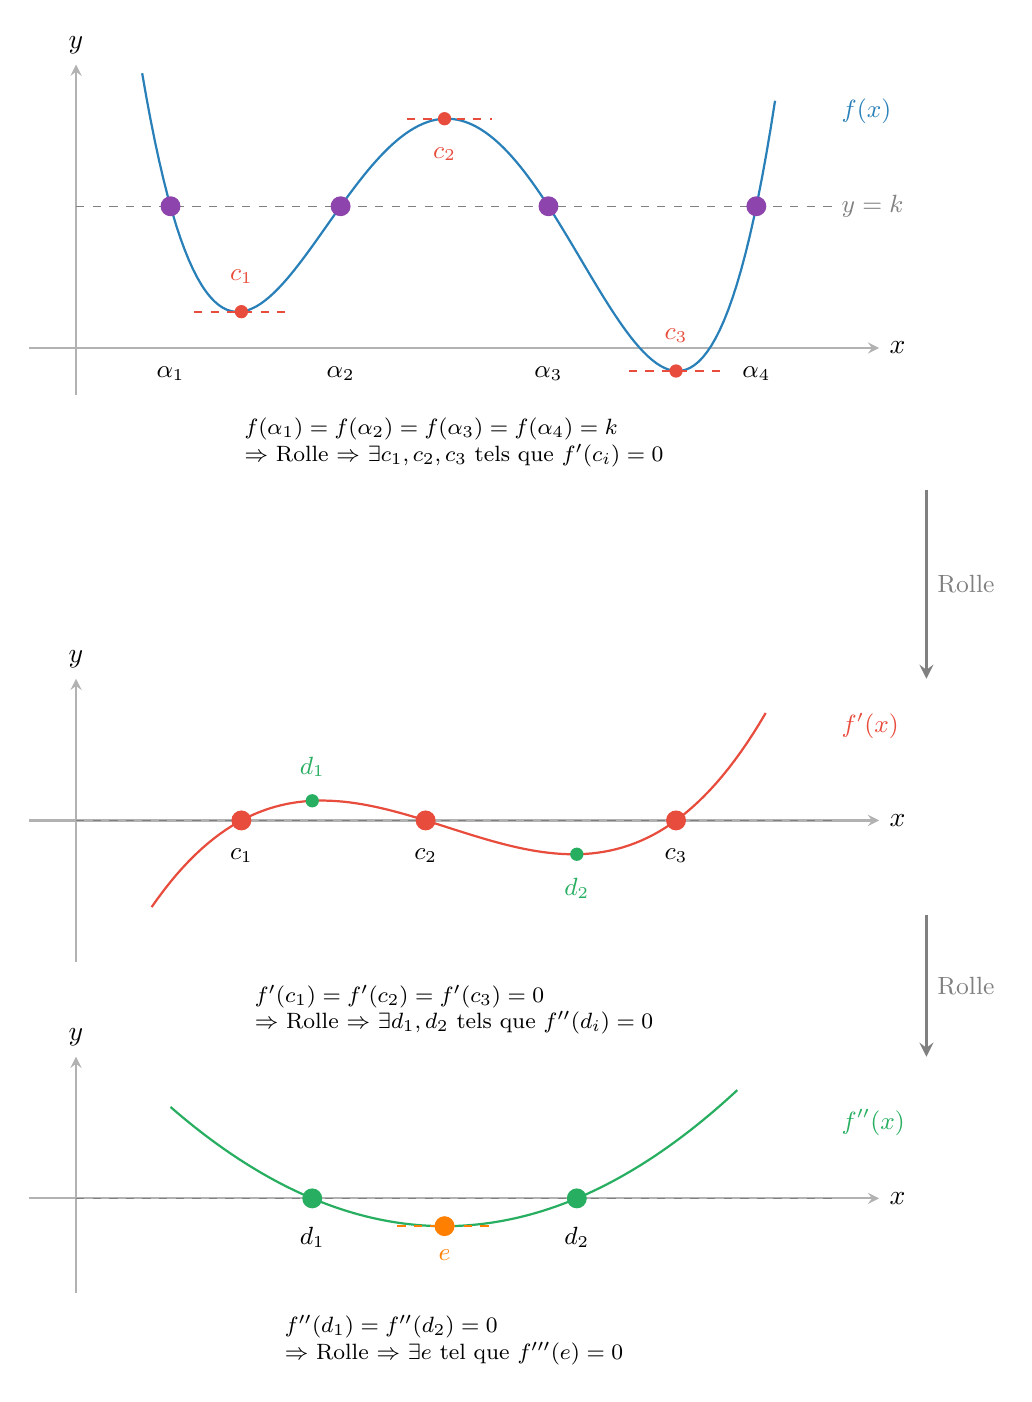
\begin{tikzpicture}[scale=1.2, >=stealth]
        % --- CONFIGURATION ---
        \definecolor{curveColor}{RGB}{41, 128, 185}
        \definecolor{derivColor}{RGB}{231, 76, 60}
        \definecolor{deriv2Color}{RGB}{39, 174, 96}
        \definecolor{pointColor}{RGB}{142, 68, 173}
        
        % Définition des points alpha
        % alpha_1 = 1, alpha_2 = 2.8, alpha_3 = 5, alpha_4 = 7.2
        % f(x) = 1.5 + 0.08*(x-1)*(x-2.8)*(x-5)*(x-7.2)
        % f'(x) = 0.08 * [(x-2.8)(x-5)(x-7.2) + (x-1)(x-5)(x-7.2) + (x-1)(x-2.8)(x-7.2) + (x-1)(x-2.8)(x-5)]
        % Simplifié: f'(x) = 0.08 * [4x^3 - 3*(1+2.8+5+7.2)x^2 + ...]
        % Les zéros de f' sont approximativement à x ≈ 1.75, 3.7, 6.35
        
        % === GRAPHIQUE 1 : f(x) avec 4 points (n=3) ===
        \begin{scope}[yshift=0cm]
            % Axes
            \draw[->, gray!60, thick] (-0.5,0) -- (8.5,0) node[right, black] {$x$};
            \draw[->, gray!60, thick] (0,-0.5) -- (0,3) node[above, black] {$y$};
            
            % Courbe f(x) = 1.5 + 0.08*(x-1)*(x-2.8)*(x-5)*(x-7.2)
            \draw[curveColor, thick, domain=0.7:7.4, samples=150] 
                plot (\x, {1.5 + 0.08*(\x-1)*(\x-2.8)*(\x-5)*(\x-7.2)});
            
            % Ligne horizontale y = k (valeur commune)
            \draw[gray, dashed] (0, 1.5) -- (8, 1.5) node[right, font=\small] {$y = k$};
            
            % Points alpha_1, alpha_2, alpha_3, alpha_4
            \foreach \x/\label in {1/$\alpha_1$, 2.8/$\alpha_2$, 5/$\alpha_3$, 7.2/$\alpha_4$} {
                \fill[pointColor] (\x, 1.5) circle (3pt);
                \node[below, font=\small] at (\x, -0.1) {\label};
            }
            
            % Points c_1, c_2, c_3 où f'=0 (positions approximatives des extremums)
            \foreach \x in {1.75, 3.9, 6.35} {
                \fill[derivColor] (\x, {1.5 + 0.08*(\x-1)*(\x-2.8)*(\x-5)*(\x-7.2)}) circle (2pt);
            }
            
            % Tangentes horizontales aux points c_i
            \draw[derivColor, dashed, thick] (1.25, {1.5 + 0.08*(1.75-1)*(1.75-2.8)*(1.75-5)*(1.75-7.2)}) -- (2.25, {1.5 + 0.08*(1.75-1)*(1.75-2.8)*(1.75-5)*(1.75-7.2)});
            \draw[derivColor, dashed, thick] (3.5, {1.5 + 0.08*(3.9-1)*(3.9-2.8)*(3.9-5)*(3.9-7.2)}) -- (4.4, {1.5 + 0.08*(3.9-1)*(3.9-2.8)*(3.9-5)*(3.9-7.2)});
            \draw[derivColor, dashed, thick] (5.85, {1.5 + 0.08*(6.35-1)*(6.35-2.8)*(6.35-5)*(6.35-7.2)}) -- (6.85, {1.5 + 0.08*(6.35-1)*(6.35-2.8)*(6.35-5)*(6.35-7.2)});
            
            % Labels pour c_i
            \node[derivColor, above, font=\small] at (1.75, {1.5 + 0.08*(1.75-1)*(1.75-2.8)*(1.75-5)*(1.75-7.2) + 0.2}) {$c_1$};
            \node[derivColor, below, font=\small] at (3.9, {1.5 + 0.08*(3.9-1)*(3.9-2.8)*(3.9-5)*(3.9-7.2) - 0.2}) {$c_2$};
            \node[derivColor, above, font=\small] at (6.35, {1.5 + 0.08*(6.35-1)*(6.35-2.8)*(6.35-5)*(6.35-7.2) + 0.2}) {$c_3$};
            
            % Annotations
            \node[curveColor, right, font=\small] at (8, 2.5) {$f(x)$};
            \node[align=left, font=\footnotesize] at (4, -1) {
                $f(\alpha_1) = f(\alpha_2) = f(\alpha_3) = f(\alpha_4) = k$\\
                $\Rightarrow$ Rolle $\Rightarrow$ $\exists c_1, c_2, c_3$ tels que $f'(c_i) = 0$
            };
        \end{scope}
        
        % === GRAPHIQUE 2 : f'(x) avec 3 zéros ===
        \begin{scope}[yshift=-5cm]
            % Axes
            \draw[->, gray!60, thick] (-0.5,0) -- (8.5,0) node[right, black] {$x$};
            \draw[->, gray!60, thick] (0,-1.5) -- (0,1.5) node[above, black] {$y$};
            
            % Courbe f'(x) = 0.32*(x-1.75)*(x-3.7)*(x-6.35) (polynôme cubique passant par les 3 zéros)
            % Facteur d'échelle ajusté pour un bon rendu visuel
            \draw[derivColor, thick, domain=0.8:7.3, samples=100] 
                plot (\x, {0.06*(\x-1.75)*(\x-3.7)*(\x-6.35)});
            
            % Ligne y = 0
            \draw[gray, dashed] (0, 0) -- (8, 0);
            
            % Points c_1, c_2, c_3 où f'=0
            \foreach \x/\label in {1.75/$c_1$, 3.7/$c_2$, 6.35/$c_3$} {
                \fill[derivColor] (\x, 0) circle (3pt);
                \node[below, font=\small] at (\x, -0.2) {\label};
            }
            
            % Points d_1, d_2 où f''=0 (entre les zéros de f')
            % Pour un cubique (x-a)(x-b)(x-c), les extremums sont aux racines de la dérivée
            % d_1 ≈ 2.5, d_2 ≈ 5.3 (approximations)
            \foreach \x in {2.5, 5.3} {
                \fill[deriv2Color] (\x, {0.06*(\x-1.75)*(\x-3.7)*(\x-6.35)}) circle (2pt);
            }
            
            % Labels pour d_i
            \node[deriv2Color, above, font=\small] at (2.5, {0.06*(2.5-1.75)*(2.5-3.7)*(2.5-6.35) + 0.15}) {$d_1$};
            \node[deriv2Color, below, font=\small] at (5.3, {0.06*(5.3-1.75)*(5.3-3.7)*(5.3-6.35) - 0.15}) {$d_2$};
            
            % Annotations
            \node[derivColor, right, font=\small] at (8, 1) {$f'(x)$};
            \node[align=left, font=\footnotesize] at (4, -2) {
                $f'(c_1) = f'(c_2) = f'(c_3) = 0$\\
                $\Rightarrow$ Rolle $\Rightarrow$ $\exists d_1, d_2$ tels que $f''(d_i) = 0$
            };
        \end{scope}
        
        % === GRAPHIQUE 3 : f''(x) avec 2 zéros ===
        \begin{scope}[yshift=-9cm]
            % Axes
            \draw[->, gray!60, thick] (-0.5,0) -- (8.5,0) node[right, black] {$x$};
            \draw[->, gray!60, thick] (0,-1) -- (0,1.5) node[above, black] {$y$};
            
            % Courbe f''(x) = A*(x-2.5)*(x-5.3) (parabole passant par les 2 zéros)
            \draw[deriv2Color, thick, domain=1:7, samples=100] 
                plot (\x, {0.15*(\x-2.5)*(\x-5.3)});
            
            % Ligne y = 0
            \draw[gray, dashed] (0, 0) -- (8, 0);
            
            % Points d_1, d_2 où f''=0
            \foreach \x/\label in {2.5/$d_1$, 5.3/$d_2$} {
                \fill[deriv2Color] (\x, 0) circle (3pt);
                \node[below, font=\small] at (\x, -0.2) {\label};
            }
            
            % Point k où f'''=0 (sommet de la parabole, au milieu)
            \fill[orange] (3.9, {0.15*(3.9-2.5)*(3.9-5.3)}) circle (3pt);
            \node[orange, below, font=\small] at (3.9, {0.15*(3.9-2.5)*(3.9-5.3) - 0.15}) {$e$};
            
            % Tangente horizontale en e
            \draw[orange, dashed, thick] (3.4, {0.15*(3.9-2.5)*(3.9-5.3)}) -- (4.4, {0.15*(3.9-2.5)*(3.9-5.3)});
            
            % Annotations
            \node[deriv2Color, right, font=\small] at (8, 0.8) {$f''(x)$};
            \node[align=left, font=\footnotesize] at (4, -1.5) {
                $f''(d_1) = f''(d_2) = 0$\\
                $\Rightarrow$ Rolle $\Rightarrow$ $\exists e$ tel que $\boxed{f'''(e) = 0}$
            };
        \end{scope}
        
        % Flèches entre les graphiques
        \draw[->, very thick, gray] (9, -1.5) -- (9, -3.5) node[midway, right, font=\small] {Rolle};
        \draw[->, very thick, gray] (9, -6) -- (9, -7.5) node[midway, right, font=\small] {Rolle};
        
    \end{tikzpicture}
    \caption{Illustration de l'exercice : Application successive du théorème de Rolle. Si $f$ prend la même valeur en $n+1 = 4$ points, alors $f'$ s'annule en $3$ points, puis $f''$ s'annule en $2$ points, et finalement $f^{(3)}$ s'annule en au moins $1$ point.}
    \label{fig:rolle_generalise}
\end{figure}

\begin{remark}
  Le résultat ci-dessus peut être utilisé en tant que théorème ou propriété de cours.
\end{remark}

\begin{application}
  Soit $f \in \mathcal{C}^2([a,b],\R)$. Montrer que $\forall t \in [a,b], \exists c \in [a,b]$ tel que $f(t)=f(a)\cdot \frac{t-b}{a-b} + f(b)\cdot \frac{t-a}{b-a} + \frac{(t-a)(t-b)}{2} f''(c)$.
\end{application}

\begin{proof}
  Si $t\in\{a,b\}$, la propriété est triviale en prenant $c=t$.

  Soit $t\in ]a,b[$.
  On définit la fonction $g : [a,b] \to \R$ par $g(x) = f(x) - f(a)\cdot \frac{x-b}{a-b} - f(b)\cdot \frac{x-a}{b-a} - \frac{(x-a)(x-b)}{2} A$ où $A$ est une constante, avec $g(t)=0$.

  On a $\begin{cases}
  g \text{ est de classe } \mathcal{C}^2 \text{ sur } [a,b]\\
  g(a) = g(b) = g(t) = 0
  \end{cases}$ (sans oublier que $t$ est \textbf{fixé}).

  Donc, d'après l'exercice précédent, il existe $c \in ]a,b[$ tel que $g''(c) = 0$.
\end{proof}

\todo{a continuer}

\section{Théorème des accroissements finis}

\begin{theorem}[Théorème des accroissements finis]
  Soit $f$ une fonction de $[a,b]\to\R$ avec $a < b$ telle que $f$ est continue sur $[a,b]$, dérivable sur $]a,b[$.

  Alors, il existe $c \in ]a,b[$ tel que $f'(c) = \frac{f(b) - f(a)}{b - a}$.
\end{theorem}

\begin{proof}
  Soient $x,y\in I$ avec $x<y$.

  On pose $g:t\mapsto (f(x)-f(y))t - f(t)(x-y)$.

  On a $\begin{cases}
  g \text{ est continue sur } [x,y]\\
  g \text{ est dérivable sur } ]x,y[\\
  g(x) = g(y)
  \end{cases}$

  Donc d'après le théorème de Rolle, il existe $c\in]x,y[$ tel que $g'(c) = 0$.

  i.e. $(f(x)-f(y)) - f'(c)(x-y) = 0$.
\end{proof}

\begin{application}
  Soit $f:I\to\R$ dérivable sur $I$ telle que $f'$ est bornée sur $I$, i.e. $\exists M\geq 0, \forall x\in I, |f'(x)| \leq M$. Donc $f$ \textbf{est lipschitzienne} sur $I$, i.e. $\forall x,y\in I, |f(x)-f(y)| \leq M|x-y|$.
\end{application}

\begin{proof}
  Soient $x,y\in I$ avec $x<y$.

  D'après le théorème des accroissements finis, il existe $c\in]x,y[$ tel que $f'(c) = \frac{f(y)-f(x)}{y-x}$.

  Donc, $|f(y)-f(x)| = |f'(c)||y-x| \leq M|y-x|$.

  Ainsi, $\forall x,y\in I, |f(x)-f(y)| \leq M|x-y|$.
\end{proof}

\begin{example}
  \begin{enumerate}
    \item Les fonctions $\cos$ et $\sin$ sont des fonctions 1-lipschitziennes sur $\R$ car leurs dérivées sont bornées par $1$.
    \item La fonction $\arctg$ est aussi 1-lipschitzienne sur $\R$ car sa dérivée est $\frac{1}{1+x^2}$, qui est bornée par $1$.
  \end{enumerate}
\end{example}

\begin{theorem}
  Soit $f \in \R^I$ une fonction continue sur $I$ et dérivable sur $\overset{\circ}{I}$.

  \begin{enumerate}
    \item $f$ est croissante sur $I$ $\iff$ $f'(x) \ge 0, \forall x \in \overset{\circ}{I}$.
    \item $f$ est décroissante sur $I$ $\iff$ $f'(x) \le 0, \forall x \in \overset{\circ}{I}$.
    \item $f$ est constante sur $I$ $\iff$ $f'(x) = 0, \forall x \in \overset{\circ}{I}$.
  \end{enumerate}
\end{theorem}

\begin{proof}
  \begin{outline}
    \1[$\implies$] Soit $x\in\overset{\circ}{I}$, $\forall y \in I-\{x\}$.
    \2 Comme $f$ est croissante sur $I$, on a $f(y) - f(x) > 0$ si $y > x$ et $f(y) - f(x) < 0$ si $y < x$.
    \2 Donc, $\frac{f(y) - f(x)}{y - x} > 0$.
    \2 Donc, en passant à la limite $y\to x$, on a $f'(x) \geq 0$.
    \2 Cela veut donc dire que $\forall x \in \overset{\circ}{I}, f'(x) \geq 0$.
    \1[$\impliedby$] Soient $x,y\in I$ avec $x<y$.
    \2 D'après le théorème des accroissements finis, il existe $c\in]x,y[$ tel que $f'(c) = \frac{f(y)-f(x)}{y-x}$.
    \2 Donc, comme $f'(c) > 0$, on a $f(y) - f(x) > 0$.
    \2 Ainsi, $f$ est croissante sur $I$.
  \end{outline}
\end{proof}

\begin{theorem}
  Soit $f \in \R^I$ continue sur $I$, dérivable sur $\overset{\circ}{I}$ et strictement croissante sur $I$.

  Cela équivaut à dire que : $\begin{cases} f'\ge 0 \text{ sur } \overset{\circ}{I} \\ A = \{x\in\overset{\circ}{I}, f'(x) = 0\} \text{ est d'intérieur vide.} \end{cases}$

  Un exemple visuel est donné dans la figure \ref{fig:croissance_derivee_nulle}.
\end{theorem}

\begin{remark}
  Une partie $A$ d'un intervalle $I$ est dite d'intérieur vide si elle ne contient pas d'intervalle non trivial, c.à.d. qu'il n'existe pas d'intervalle $[c,d] \subset I$ avec $c < d$ tel que $[c,d] \subset A$.
\end{remark}

\begin{proof}
  \begin{itemize}
    \item Démonstration triviale dans le sens direct.
    \item Réciproquement, supposons que $f'\ge 0$ sur $\overset{\circ}{I}$, que $A = \{x\in\overset{\circ}{I}, f'(x) = 0\}$ est d'intérieur vide et que $f$ est croissante sur $I$.\\i.e. $\forall a<b \in I, f(a) \le f(b)$.\\Si $\exists a<b\in I, f(a) = f(b)$, alors d'après le théorème de Rolle, $\exists c\in]a,b[$ tel que $f'(c) = 0$. Donc $c\in A$.\\Comme $f$ est croissante sur $I$, on a $\forall x\in]a,b[, f(a) \le f(x) \le f(b)$, donc $f(x) = f(a)$, i.e. $]a,b[ \subset A$, ce qui contredit le fait que $A$ est d'intérieur vide.\\Donc, $\forall a<b \in I, f(a) < f(b)$, i.e. $f$ est strictement croissante sur $I$.
  \end{itemize}
\end{proof}

\begin{figure}[H]
    \centering
    \begin{tikzpicture}
        \begin{axis}[
            width=12cm, height=8cm,
            axis lines=middle,
            grid=both,
            grid style={line width=.1pt, draw=gray!20},
            major grid style={line width=.2pt,draw=gray!50},
            xmin=-0.8, xmax=3.8,
            ymin=-0.5, ymax=2.8,
            xlabel=$x$, ylabel=$y$,
            legend style={at={(0.05,0.95)}, anchor=north west},
            samples=200,
            domain=-0.8:3.8
        ]
            % Fonction f(x) = cos((x + 0.5)*2*pi) + 1
            % C'est la dérivée (à un facteur près) qui s'annule aux entiers
            \addplot[
                color=teal,
                thick,
                smooth
            ]
            {cos(deg((x + 0.5)*2*pi)) + 1};
            \addlegendentry{$f'(x) = \cos(2\pi(x+\frac{1}{2})) + 1$}

            % Fonction g(x) = (1/(2*pi)) * sin((x + 0.5)*2*pi) + x
            % C'est la fonction strictement croissante dont la dérivée s'annule
            \addplot[
                color=mainBlue,
                very thick,
                smooth
            ]
            {(1/(2*pi)) * sin(deg((x + 0.5)*2*pi)) + x};
            \addlegendentry{$f(x) = \frac{1}{2\pi}\sin(2\pi(x+\frac{1}{2})) + x$}

            % Points où la dérivée s'annule (tangentes horizontales)
            \addplot[only marks, mark=*, color=mainBlue, mark size=2pt] coordinates {
                (0,0) (1,1) (2,2) (3,3)
            };
            
            % Tangentes horizontales (visuel)
            \draw[mainBlue, thick, opacity=0.5] (axis cs:-0.3,0) -- (axis cs:0.3,0);
            \draw[mainBlue, thick, opacity=0.5] (axis cs:0.7,1) -- (axis cs:1.3,1);
            \draw[mainBlue, thick, opacity=0.5] (axis cs:1.7,2) -- (axis cs:2.3,2);
            \draw[mainBlue, thick, opacity=0.5] (axis cs:2.7,3) -- (axis cs:3.3,3);

        \end{axis}
    \end{tikzpicture}
    \caption{Illustration d'une fonction $g$ strictement croissante sur $\mathbb{R}$ (en bleu) dont la dérivée $f'(x)$ (en vert) s'annule pourtant une infinité de fois (pour tout $n \in \mathbb{N}$). Cela montre que $f' > 0$ n'est pas une condition nécessaire pour la stricte croissance, $f' \ge 0$ et ne s'annulant pas sur un intervalle suffit.}
    \label{fig:croissance_derivee_nulle}
\end{figure}

\begin{theorem}[Théorème des accroissements finis généralisé]
  Soient $f,g : I \to \R$ deux fonctions continues sur $I$, dérivables sur $\overset{\circ}{I}$, telles que $\abs{f'} \le g'$ sur $\overset{\circ}{I}$.

  Alors, $\forall x,y \in I, \abs{f(x)-f(y)} \leq \abs{g(x)-g(y)}$.
\end{theorem}

\begin{proof}
  Soient $x<y \in I$. (Le cas $x>y$ se traite de la même manière, sans perte de généralité).

  On a $-g'\le f' \le g'$ sur $\overset{\circ}{I}$.
  Donc $\begin{cases}
\forall t \in \overset{\circ}{I}, f'(t) + g'(t) \ge 0 \\ \forall t \in \overset{\circ}{I}, g'(t) - f'(t) \ge 0
\end{cases}$

  Donc $\begin{cases}
    f(x) - f(y) + g(x) - g(y) \ge 0 \\ g(x) - g(y) - (f(x) - f(y)) \ge 0
  \end{cases}$

  Donc $\begin{cases}
    f(x) - f(y) \ge -(g(x) - g(y)) \\ f(x) - f(y) \le g(x) - g(y)
  \end{cases}$

  Donc, $\abs{f(x) - f(y)} \leq \abs{g(x) - g(y)}$.

  Donc, $\forall x,y \in I, \abs{f(x)-f(y)} \leq \abs{g(x)-g(y)}$.
\end{proof}

\begin{consequence}
  Soit $f \in \R^I$ une fonction continue sur $I$, dérivable sur $\overset{\circ}{I}$ telle que $f'$ est bornée sur $\overset{\circ}{I}$, i.e. $\exists M\geq 0, \forall x\in \overset{\circ}{I}, |f'(x)| \leq M$. Alors, $\forall x,y \in I, \abs{f(x)-f(y)} \leq M \abs{x-y}$.
\end{consequence}

\begin{proof}
  On prend $g: I \mapsto M\cdot x$ et on applique le théorème des accroissements finis généralisé.

  \begin{itemize}
    \item On a $g'(x) = M$.
    \item Donc, $\abs{f'(x)} \leq M = g'(x)$.
    \item Donc, d'après le théorème des accroissements finis généralisé, $\forall x,y \in I, \abs{f(x)-f(y)} \leq \abs{g(x)-g(y)} = M\abs{x-y}$.
  \end{itemize}

  Ainsi, $\forall x,y \in I, \abs{f(x)-f(y)} \leq M \abs{x-y}$.
\end{proof}

\begin{consequence}
  Soit $f \in \R^I$ une fonction continue sur $I$, et de classe $\mathcal{C}^1$ sur $\overset{\circ}{I}$, alors :

  $$\forall x,y \in \overset{\circ}{I}~|~x<y, \abs{f(y)-f(x)} \leq \sup_{t\in[x,y]} |f'(t)| \cdot |y-x|.$$
\end{consequence}

\begin{proof}
  On sait que $f$ est de classe $\mathcal{C}^1$ sur $\overset{\circ}{I}$, donc $f'$ est continue sur $\overset{\circ}{I}$, donc sur $[x,y]$.

  On en déduit donc que $f'$ est bornée sur $[x,y]$ et qu'elle atteint ses bornes (l'image d'un segment par une fonction continue est un segment).

  On applique donc le théorème des accroissements finis généralisé.
\end{proof}

\begin{theorem}[Prolongement de la dérivée]
    Soit $f:[a,b]\to\R$ telle que :

    $\begin{cases}
        f \text{ est continue sur } [a,b]\\
        f \text{ est dérivable sur } [a,b[\\
        \lim_{x\to b^-}f'(x)=l\in\R
    \end{cases}$

    Alors $f$ est dérivable en $b$ avec $f'(b)=l$.
\end{theorem}

\begin{proof}
    Pour démontrer ce théorème, nous devons montrer que $\lim_{x\to b^-}\frac{f(x)-f(b)}{x-b} =l$.

    \begin{itemize}
        \item On sait que $\lim_{x\to b^-}f'(x)=l$.

        \item Donc $\forall \eps > 0, \exists c \in [a,b[, \forall x \in [c,b[ : \abs{f'(x)-l}<\eps$.

        \item Soit $x\in[c,b[$, i.e. $x<b$.
    
        \item Comme $f$ est continue sur $[x,b]$, dérivable sur $]x,b[$.
    
        \item Alors, en appliquant le théorème des accroissements finis, $\exists d \in ]x,b[ : f'(d)=\frac{f(x)-f(b)}{x-b}$.
    
        \item On a $d \in ]x,b[ \implies d\in [c,b[$.
    
        \item Donc $\abs{f'(d)-l} < \eps \implies \abs{\frac{f(x)-f(b)}{x-b} -l} < \eps$.
    \end{itemize}

    On conclut que $\lim_{x\to b^-} \frac{f(x)-f(b)}{x-b}=l\in\R$, i.e. $f$ est dérivable en $b$ avec $f'(b)=l$.
\end{proof}

\begin{remark}
    \begin{enumerate}
        \item $f$ est dérivable en $b$ $\nimplies$ (n'implique pas)
        \item Si $f:[a,b]\to \R$ telle que\\$\begin{cases}
            f \text{ est continue sur } [a,b]\\
            f \text{ est } \mathcal{C}^1 \text{ sur } [a,b[\\
            \lim_{x\to b^-}f'(x)=l
        \end{cases}$\\Alors $f$ est de classe $\mathcal{C}^1$ sur $[a,b]$.
    \end{enumerate}
\end{remark}
\todo{à continuer (1)}

\begin{theorem}[Généralisation du prolongement]
    Soit $f : [a,b] \to \R$ telle que :

    $\begin{cases}
        f \text{ est continue sur } [a,b]\\
        f \text{ est de classe } \mathcal{C}^n \text{ sur } [a,b[\\
        \forall k \in [\![1,n]\!], \lim_{x \to b^-} f^{(k)}(x)=l_k\in\R
    \end{cases}$

    Alors $f$ est de classe $\mathcal{C}^n$ sur $[a,b]$ avec $\forall k \in [\![1,n]\!]: f^{(k)}(b)=l_k$.

    La démonstration de ce théorème se fait par récurrence sur $n\in\N^*$.
\end{theorem}

\begin{exercise}
    Soit $f:x\mapsto \begin{cases} e^{\frac{-1}{x^2}}, x\not=0\\0~~ , x=0\end{cases}$.

    \textbf{Solution :}

    \begin{itemize}
        \item On a $f$ est de classe $\mathcal{C}^n$ sur $\R_+^*$ et $\R_-^*$.
        \item On a $\lim_{x\to 0}f(x)=\lim_{x\to 0}e^{-\frac1{x^2}}=0=f(0)$.
        \item Donc $f$ est continue en $0$.
        \item placeholder
        \item avec $P_{n+1}(x)=\underbrace{2x^3P_n(x)}_{d^\circ = 3n+3}-\underbrace{x^2P_n'(x)}_{d^\circ=3n+1}$.
        \item Donc $d^\circ P_{n+1}=3(n+1)$.
        \item Donc on a $\forall n \ge 1, \forall x \neq 0, f^(n)(x)=P_n(\frac{1}{x})e^{-\frac{1}{x^2}}$.
        \item Alors $\lim_{x\to0} f^{(n)}(x)=\lim_{t\to\infty}P_n(t)e^{-t^2}$.
        \item Donc $\lim_{x\to0} f^{(n)}(x)=0 \in \R$, et ce, pour tout $n\ge 1$.
    \end{itemize}

    On conclut que $f$ est de classe $\mathcal{C}^\infty$ sur $\R$ avec $\forall n \in \N, f^{(n)}(0)=0$.
\end{exercise}
\todo{erm remove placeholder}

\begin{theorem}[Formule de Taylor-Lagrange]
    Soit $f \in \mathcal{C}^n(I,\R) \cap D^{n+1}(\overset{\circ}{I},\R)$.

    Alors $\forall a \in I, \forall x \ne a, \exists c \in ]\min(a,x),\max(a,x)[$ tel que :

    $$f(x)=\sum_{k=0}^n\parens{\frac{f^{(k)}(a)}{k!}(x-a)^k}+\frac{f^{(n+1)}(c)}{(n+1)!}(x-a)^{n+1}$$
\end{theorem}

\begin{proof}
    Soient $a\in I, x\ne a$.

    On pose $g:t\mapsto f(x)-\sum_{k=0}^n f^{(k)}(t)(x-t)^k-A(x-t)^{n+1}$ où $A$ est une constante telle que $g(a)=0$.
\end{proof}
\todo{a continuer}

Cette méthode utilisée dans les démonstrations précédentes doit devenir un quasi-réflexe pour la résolution d'exercices où des dérivées dépendent d'un certain $c$ existant dans [...].

\begin{remark}
    Pour $n=0$, on retrouve la formule du théorème des accroissements finis.
\end{remark}

\begin{consequence}[Inégalité de Taylor-Lagrange]
    Soit $f \in \mathcal{C}^{n+1}(I,\R)$. 

    On a, pour tout $x\ne a \in I$ :

    $$\abs{f(x)-\sum_{k=0}^n\frac{f^{(k)}}{k!}(x-a)^k}\le\sup_{t\in[a,x] \text{ ou }t \in [x,a]}\abs{f^{(n+1)}(t)}\frac{\abs{x-a}}{(n+1)!}$$

    La démonstration se fait en utilisant la formule de Taylor-Lagrange, et en utilisant le fait que $f$ est de classe $\mathcal{C}^{n+1}$ sur $I$, donc $\abs{f^{(n+1)}(c)}\le \sup_{t\in[a,x]\text{ ou } t\in[x,a]}\abs{f^{(n+1)}(t)}$.
\end{consequence}

\chapter{Convexité}

\begin{definition}
    Soit $f \in \R^I$ telle que $I$ est un intervalle de $\R$ avec $\overset{\circ}{I}\ne\emptyset$.

    \begin{enumerate}
        \item $f$ est dite \textbf{convexe} sur $I$ si et seulement si $\forall t \in [0,1], \forall x,y \in I$\\$$f(tx+(1-t)y\le tf(x)+(1-t)f(y)$$
        \item $f$ est dite \textbf{concave} si et seulement si $-f$ est concave, donc si et seulement si $\forall t \in [0,1], \forall x,y \in I$\\$$f(tx+(1-t)y\ge tf(x)+(1-t)f(y)$$
    \end{enumerate}
\end{definition}

\begin{remark}
    Soient $x,y \in I$ tels que $x<y$.

    On pose $\varphi : \begin{cases} [0,1]\to[x,y]\\t\mapsto tx+(1-t)y \end{cases}$
\end{remark}
\todo{recop}

\begin{property}[Inégalité de Jensen]
    Soit $f \in \R^I$ convexe sur $I$.
    
    Alors, $\forall n \ge 1, \begin{cases} \forall \lambda_1,\dots,\lambda_n\in[0,1]~|~\sum_{i=1}^n\lambda_i=1\\ \forall x_1,\dots,x_n \in I\end{cases}$

    $$f\parens{\sum_{i=1}^n\lambda_i x_i}\le \sum_{i=1}^n \lambda_i\cdot f(x_i)$$
\end{property}

\begin{proof}
    On procède par récurrence sur $n\in\N^*$.

    \begin{outline}
        \1 Pour $n=1$, on a $f(x)\le f(x)$. Pour $n=2$, on obtient la définition de la convexité.

    \1 Soit $n\ge 1$, supposons que le résultat est vrai au rang $n$.

    \2 Soient $\begin{cases}
        \lambda_1,\dots,\lambda_n \in [0,1]~|~\sum_{i=1}^{n+1}\lambda_i=1
        \\
        x_1,\dots,x_{n+1}\in I
    \end{cases}$

    \2 On pose $t=\sum_{i=1}^n \lambda_i \implies \lambda_{n+1} = 1-t$

    \2 Dans le cas où $t=0$, alors $\lambda_{n+1}=1, \forall n \in [\![1,n]\!], d_i=0$.

    \2 Cela implique que $f\parens{\sum_{i=1}^{n+1}\lambda_i x_i}=f(x_{n+1})\le f(x_{n+1}) = \sum_{i=1}^{n+1} \lambda_i f(x_i)$
    \end{outline}
\end{proof}

\end{document}

